\section{Suunnitelu}
Tarkoituksena oli tehdä sulautettu laite joka
\begin{itemize}
  \item voi ohjata LEDiä
  \item voidaan liittää verkkoon
  \item mahdollistaa LEDin ohjauksen verkkosivun kautta tai fyysistä nappia
    painamalla.
\end{itemize}
Vaatimuksena oli myös että piirilevy on itsetehty ja että siinä käytetään
mikrokontrolleria joka yhdistetään nettiin jonkunlaisen modeemin kautta
käyttäen AT-komentoja. Valitettavasti en itse ollut tietoinen tästä viimeisestä
vaatimuksesta, vaan ohjelmoin ESP8266 piirin suoraan. Tämän seurauksena
selostuksessa on puoli sivua ylimääräistä kohdassa~\ref{sec:extra}. Huomaamatta
jäi myös vaatimus fyysisestä painonapista, mutta sen lisääminen ei
onneksi ollut kovin iso työ.

Heti kun kuulin harjoitustyöstä halusin kokeilla käyttää ESP8266 moduulia
itsenäisesti ilman ohjaavaa mikrokontrolleria. Halusin myös ohjelmoida piirin
suoraan, enkä käyttää välissä käyttöjärjestelmää tai kolmannen osapuolen
firmwarea, kuten esimerkiksi NodeMcu:ta.\cite{nodemcu}

Syy tähän oli se että olin jo pitkään halunnut tutustua ESP8266 piiriin, mutten
ollut löytänyt sille aikaa. Halusin siis käyttää harkkatyön mahdollisimman
hyvin hyödyksi, ja uskoin että laitteistonläheinen C ja alustan tuomat
rajoitukset olisivat opettavaisia. Tykkään myös pyrkiä projekteissani
yksinkertaisuuteen aina kun se on mahdollista ja/tai järkevää. Halusin myös
tehdä mahdollisimman uudelleenkäytettävän piirilevyn, jotta sen hyödyllisyys ei
rajoittuisi tähän kurssiin.

Nettisivua en suunnitellut etukäteen yhtä tarkasti kuin piirilevyä. Alusta asti
oli kuitenkin selvää että toteutus olisi mahdollisimman yksinkertainen, mikä
tarkoittaisi luultavasti PHP:llä toteutettua backend-sovellusta.

\section{Piirilevy ja komponentit}
Päädyin käyttämään työssäni ESP-12E moduulia oikeastaan siitä syystä että sain
ostettua sellaisen lähipiiristäni. Oikeitakin syitä tämän moduulin
valitsemiselle kuitenkin on. Siinä on aikaisempia malleja enemmän liitäntöjä
piiriin (SPI ja 2 GPIO:ta lisää), piirillä on RF-häiriöitä vähentävä suojakuori
ja piirille on kuparivedoilla tehty pieni antenni, joka ainakin periaatteessa
parantaa moduuliin lähetys- ja vastaanottotehoja. Täytyy kuitenkin lisätä tähän
että loppujen lopuksi ainakin useimmissa harraste- ja kurssiprojekteissa eri
moduulien välillä ei ole huomattavia eroja.

Koska en käyttänyt työssäni erillistä mikrokontrolleria, jäi piirilevyni
erittäin yksinkertaiseksi. Itse jakaisin suunnittelemani piirin toiminnoiltaan
kolmeen osaan:
\begin{itemize}
  \item Moduulin liitäntöjen tarjoaminen piikkirimoilla
  \item Nappi resetointia varten ja kytkin piirin boottaustilan vaihtamiseksi
    flash-ohjelmoinnin ja flashista boottamisen välillä
  \item Virransyöttö
\end{itemize}

Koska itse halusin tehdä piirilevyn jota voisin käyttää myös kurssin jälkeen,
oli suhteellisen tärkeää että mahdollisimman moniin moduulin liitännöistä
pääsisi kätevästi käsiksi. Pinnirimoja on 3:
\begin{itemize}
  \item UART yhteyteen tarvittavat liitännät (mukaanlukien maa ja +3.3V ja +5V
    jännitteet)
  \item GPIO:t
  \item SPI liitännät
\end{itemize}

Omassa piirissäni on kytkin toimintatilan vaihtamiseen ja reset-nappi.
ESP8266 piirin toimintatila määräytyy sen perusteella missä jännitteessä
(maassa vai käyttöjännitteessä) tietyt piirin liitännät ovat. Tässä
harjoitustyössä ja useimissa projekteissa relevantit tilat ovat flash-muistin
ohjelmointitila ja flash-muistiin ohjelmoidun ohjelman ajaminen (boot from
flash). Kuvassa~\ref{fig:esp-tila-pinnit} on esitetty kyseiset liitännät ja
niiden kytkennät.
\begin{figure}[H]
  \centering
  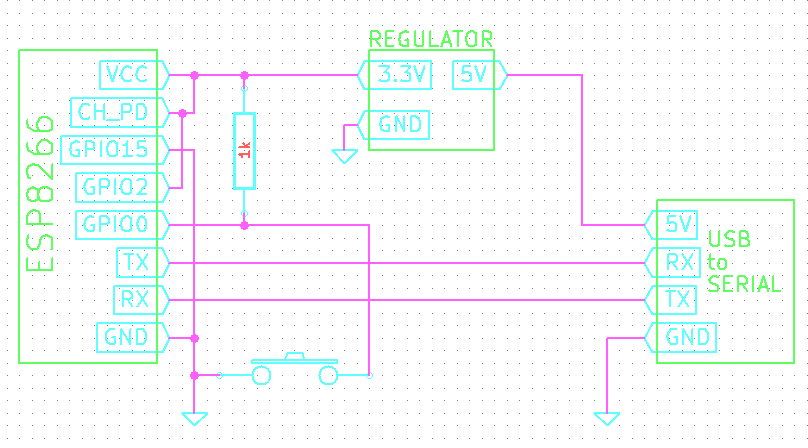
\includegraphics[width=0.8\linewidth]{esp-mode-setup}
  \caption{Kytkentä jossa napilla voidaan valita ohjelmoinnin ja boot-from-flash:n
    välillä~\cite{hackaday}}
\label{fig:esp-tila-pinnit}
\end{figure}

Virtalähteenä piirissäni on 9V paristo. Valitsin tämän pariston koska siihen
löytyy yksinkertainen ja yleinen liitäntä, ja koska +9V saa helposti laskettua
haluttuun +3.3V (ja +5V) jännitteeseen, jolloin tarvetta vaikkapa hakkurille
tai useammlle paristolle ei ole. Jännitteen reguloinnissa on käytetty LM317T
säädettävää lineaariregulaattoria. Regulaattorin ulos- ja sisääntulossa on
\(1\mu{}F\) kondensaattori ja lisäksi ESP-12 moduulin virtapinnien vieressä on
\(33\mu{}F\) kondensaattori (joka lienee hieman ylimitoitettu).

Kuvassa~\ref{fig:piiri-etu} on kuva piirilevyn etupuolesta, jossa näkyy hyvin
virransyötön komponentit (konkat, regulaattori ja paristoliitäntä) ja
piikkirimat. Vasemmalla ylhäällä on UART:tiin tarvitta piikkirima, sen
alapuolella SPI rima ja oikealla GPIO rima. Kuvassa~\ref{fig:piiri-taka} on
piirilevyn toinen puoli. Tällä puolella on itse ESP moduuli, reset-nappi ja
boottaustilan muuttava kytkin. Kuvassa~\ref{fig:nappi-ja-paristo} on piirilevyn
etupuoli ja LEDin tilaa muuttava ad-hoc painonappi ja teholähteenä toimiva
paristo.
\begin{figure}[H]
\centering
\begin{minipage}{.5\textwidth}
  \centering
  \includegraphics[width=0.9\linewidth]{front}
  \caption{Piirilevyn etupuoli}
\label{fig:piiri-etu}
\end{minipage}%
\begin{minipage}{.5\textwidth}
  \centering
  \includegraphics[width=0.9\linewidth]{back}
  \caption{Piirilevyn takapuoli}
\label{fig:piiri-taka}
\end{minipage}
\end{figure}
\begin{figure}[H]
  \centering
  \includegraphics[width=0.8\linewidth]{nappi-ja-paristo}
  \caption{Piirilevyn etupuoli pariston ja napin kera}
\label{fig:nappi-ja-paristo}
\end{figure}

\section{Ohjelmisto}
Ohjelmisto koostuu itse sulautetun laitteen ohjelmistosta, nettisivusta jonka
kautta käyttäjä näkee ja voi muuttaa LEDin tilan ja web API:sta jonka kautta
ESP tai nettisivun JavaScript koodi voi lukea tai muuttaa LEDin tilan.

\subsection{Nettisivun ja API:n ohjelmointi}
Nettisivun käyttäjäpuoli on yksinkertainen sivu, jossa lukee LEDin nykyinen
tila ja nappi mistä tilaa voi muuttaa. Sivu on perus HTML koodia, sillä
erotuksella että LEDin tilan lukeminen ja muuttaminen tehdään AJAX~\cite{ajax}
tekniikalla, mikä siis tarkoittaa sitä että tiedonsiirto tehdään asynkronisesti
JavaScript koodilla, jolloin sivua ei tarvitse päivittää kun LEDin tila
päivittyy. LEDin tila haetaan HTTP:n GET-pyynnöllä ja muutetaan POST-pyynnöllä.
Molempiin voisi tietenkin käyttää GET:iä, mutta olen sitä mieltä että kun HTTP
tarjoaa erikseen pyynnön tiedon lähettämiseen palvelimelle, tulisin tietoa
lähettäessä käyttää sitä.

Palvelimen puolella on PHP-skripti, joka lähetetyn pyynnön tyypistä (GET vai
POST) riippuen joko palauttaa LEDin tilan tai päivittää sen. LEDin tila
palautetaan formaatilla ``[led\_state]1'' tai ``[led\_state]0''.
``[led\_state]'' rimpsu helpottaa viestin jäsennystä ESP:n ohjelmiston
puolella. Itse käytin WWW-palvelimena NGINX palvelinta.

\subsection{ESP8266:n ohjelmointi}
Käytin ohjelmoinnissa hyväkseni esp-open-sdk~\cite{esp-open-sdk} nimistä
projektia. Projekti sisältää kääntäjän ja ohjelmointityökalun, jotka ovat
molemmat avointa lähdekoodia. Projektin mukana tulee myös Espressif:n SDK, joka
siis sisältää ESP8266:n ohjelmoinnissa tarvittavat rajapinnat.

Varsinkin ohjelmoinnissa tulee ottaa huomioon muutamia teknisiä yksityiskohtia
jotka liittyvät piirin ominaisuuksiin. Käsittelen näitä tarkemmin
kohdassa~\ref{sec:extra}.

ESP8266:n ohjelmointi tehdään laitteistonläheistä C:tä käyttäen. Espressif:n
tarjoama kirjasto hoitaa suuren osan verkkoliikenteen yksityiskohdista, ja
tarjoaa yksinkertaisen API:n esimerkiksi langattomaan verkkoon yhdistämistä ja
TCP ja UDP yhteyksien käsittelemistä varten. Main-funktio ja kontrollerin
hallintasilmukka on myös täysin kirjaston hallussa. Kirjasto mahdollistaa oman
koodin lisäämisen määrittelemällä \texttt{user\_init()} funktion, jonka
ohjelmoija voi toteuttaa.  Tässä funktiossa voi sitten lisätä erilaisia
callbackkeja eri tapahtumille, mm.  ``Yhdistetty verkkoon'', ``TCP yhteys
muodostettu'', ``Yhteys katkesi'' jne.  Tarvittaessa voi myös luoda ajastimia
joihin voi liittää callbackkeja, jos on tarve säännöllisille toimille.

Omassa ohjelmassani käytän sekä ajastin- että tapahtumapohjaisia callbackkeja.
Langattomaan verkkoon yhdistäminen sekä itse palvelimeen yhdistäminen ja
HTTP-pyynnön lähettäminen perustuu tapahtumiin reagoimiseen. Ensin tietenkin
yhdistetään langattomaan verkkoon. Olen kuullut toteutuksista, joissa ESP luo
käynnistyessään ensin oman ad hoc verkkonsa. Käyttäjän yhdistäessä tähän
verkkoon ESP esittää käyttäjälle web-käyttöliittymän, jossa käyttäjä voi antaa
verkon tiedot johon ESP:n halutaan yhdistävän. Itselläni toteutus oli aika
paljon yksinkertaisempi; Verkon SSID ja salasana on kovakoodattu koodiini.
Itse verkkoon liittyminen käy muutamalla rivillä:
\begin{lstlisting}[language=C]
    struct station_config stationConf;
    wifi_set_opmode( STATION_MODE );
    os_memcpy(&stationConf.ssid, wifi_ssid, 32);
    os_memcpy(&stationConf.password, wifi_passwd, 32);
    wifi_station_set_config(&stationConf);
    wifi_set_event_handler_cb(wifi_connected);
    wifi_station_connect();
\end{lstlisting}
Kun ESP on yhdistänyt verkkoon, päästään \texttt{wifi\_connected} callbackkiin,
jossa ensimmäisenä selvitetään palvelimen IP-osoite \texttt{gethostbyname}
funktion avulla, jonka jälkeen yhdistetään serveriin TCP-yhteydellä, lähetetään
HTTP-pyyntö, ja käsitellään palvelimen vastaus. Jokainen näistä toiminnoista
käsitellään omassa funktiossaan, joka rekisteröidään callbackkinä sitä
edeltävässä. Selvennyksenä esimerkki: Kun TCP-yhteys on luotu, siirrytään
``Yhdistetty palvelimeen'' tapahtumalle rekisteröityyn callbackkiin, jossa
rekisteröidään callback ``Palvelin vastasi'' tapahtumalle, ja lähetetään
HTTP-pyyntö palvelimelle. HTTP-pyynnön lähetyksen jälkeen yhteys katkeaa.

Ajastimen callback tarkistaa fyysisen napin tilan, varmistaa että LEDin
todellinen tila vastaa haluttua tilaa (ja tarvittaessa muuttaa sitä) sekä
seuraa onko yhteys palvelimeen vielä olemassa. Kuten mainitsinkin yllä, ESP:n
SDK kirjastossa on myös mahdollisuus registeröidä callback ``Yhteys katkesi''
-tapahtumaan. Jostain syystä se ei kuitenkaan toiminut täysin odotetusti:
Jonkun aikaa tapahtumaketju \texttt{yhdistä \(\rightarrow{}\) lähetä pyyntö
\(\rightarrow{}\) yhdistä uudelleen} toimii, mutta aina jonkun ajan päästä
ohjelma lakkaa yhdistämästä uudelleen, enkä valitettavasti keksinyt miksi.
Myöskään HTTP:n ``keep-alive'' yhteysparametri ei jostain syystä toiminut
odotetusti, joten tyydyin (epätäydelliseen ja luultavasti tehottomaan)
ajastinratkaisuun.

\section{ESP8266 moduulin käyttäminen ilman mikrokontrolleria}
\label{sec:extra}

Ensimmäinen erityispiirre joka täytyy huomioida ESP:tä ohjelmoitaessa juontaa
juurensa laitteen käyttö-tarkoituksesta; Laite on ensisijaisesti tarkoitettu
verkkoyhteyksien hallinnointiin, jotka vaativat säännöllisiä toimenpiteitä.
Siksi ohjelman suoritus ei saa viettää liikaa aikaa omassa koodissa, vaan
SDK-koodille tulee antaa tarpeeksi paljon aikaa hoitaa verkkoliikennettä.
Dokumentaation mukaan ohjelmoijan toteuttamissa funktioissa saa maksimissaan
käyttää 10ms suoritusaikaa. Tämä osaltaan johtaa koodiin joka perustuu lähinnä
callbackkeihin jotka suoritetaan tapahtumien ja ajastimien tahdissa. Omassa
koodissani melkein kaikki funktiot olivat callbackkeja, mikä voi olla aluksi
hieman hämmentävää, ja joka tekee debuggauksesta tietenkin vähän vaikeampaa.

Toinen erityispiirre ESP:n ohjelmoinnissa on laitteen pieni käytettävissä oleva
IRAM (Instruction RAM). IRAM on siis muistia johon ajettavan ohjelman funktiot
ladataan laitteen käynnistyessä. IRAM:ia on piirissä yhteensä 32 kilotavua,
mutta tästä on ohjelmoijan käytössä kuitenkin vain pieni osa, käsittääkseni
noin 2--3 kilotavua, koska iso osa kirjaston koodista ajetaan IRAM:sta. Näin
pieni tila funktioille tekisi monimutkaisemmasta toiminnallisuudesta
mahdotonta, mutta onneksi piirin flash-muisti on tarpeeksi nopeaa että funktiot
voidaan ajaa sieltä käsin. Jotta piiri osaa ajaa funktion flash-muistista, se
täytyy merkitä macrolla \texttt{ICACHE\_FLASH\_ATTR} Pienen tilan takia
käytännössä kaikki omat funktiot tulee merkitä kyseisellä macrolla, mutta
poikkeuksiakin on; Tietääkseni funktioita joissa käsitellään flash-muistia ei
voi ajaa sieltä.  Jostain syystä (jota ei dokumentaatiossa selitetä) macroa ei
myöskään saa käyttää ajastincallbackissä.  Voi myös olla tilanteita joissa
kuitenkin tarvitaan IRAM:ia sen nopeuden takia.  Sivuhuomiona voi todeta että
tämä macro ja sen kriittinen tarpeellisuus on melko huonosti dokumentoitu;
Ainoa syy miksi itse tiedän siitä on google-haulla löytämäni foorumiviesti,
virallisesta dokumentaatiosta en löytänyt sille selitystä.

\section{Yhteenveto}

Projektin aikana törmäsin kuitenkin pariin suunnitteluvirheeseen:
\begin{itemize}
  \item Pienellä vaivalla olisin voinut lisätä piirille USB-to-UART piirin ja
    USB liittimen, joka olisi tehnyt ohjelmoinnista todella paljon helpompaa.
    Lisää tästä kohdassa~\ref{sec:extra}
\end{itemize}
